\documentclass{article}
\usepackage[UTF8]{ctex}
\usepackage{pythonhighlight}
\usepackage{markdown}
\usepackage{listings}
\lstset{
    basicstyle          =   \tt,          % 基本代码风格
    identifierstyle=\color{brown!80!black},
    keywordstyle        =   \color{purple}\bfseries,          % 关键字风格
    commentstyle        =   \rmfamily\itshape,  % 注释的风格,斜体
    stringstyle         =   \ttfamily,  % 字符串风格
    flexiblecolumns,                % 别问为什么,加上这个
    numbers             =   left,   % 行号的位置在左边
    showspaces          =   false,  % 是否显示空格,显示了有点乱,所以不现实了
    numberstyle         =   \zihao{-5}\ttfamily,    % 行号的样式,小五号,tt等宽字体
    showstringspaces    =   false,
    captionpos          =   t,      % 这段代码的名字所呈现的位置,t指的是top上面
    frame               =   lrtb,   % 显示边框
    backgroundcolor=\color[RGB]{245,245,244},
}


% Language setting
% Replace `english' with e.g. `spanish' to change the document language
\usepackage[english]{babel}
\usepackage{float}
% Set page size and margins
% Replace `letterpaper' with `a4paper' for UK/EU standard size
\usepackage[letterpaper,top=2cm,bottom=2cm,left=3cm,right=3cm,marginparwidth=1.75cm]{geometry}

% Useful packages
\usepackage{amsmath}
\usepackage{graphicx}
\usepackage[colorlinks=true, allcolors=blue]{hyperref}

\title{数逻实验报告Lab12}
\author{雷远航}

\begin{document}

\maketitle

\begin{abstract}
    计数器、定时器设计与应用
\end{abstract}

\section*{一、操作方法与实验步骤}
\subsection*{任务1:完成同步四位二进制计数器74LS161}
根据课件上的实验原理,利用verilog完成同步二进制计数器74LS161的设计,
以便后续时钟的设计.
完成的74LS161的代码如下:
\begin{figure}[H]
    \centering
    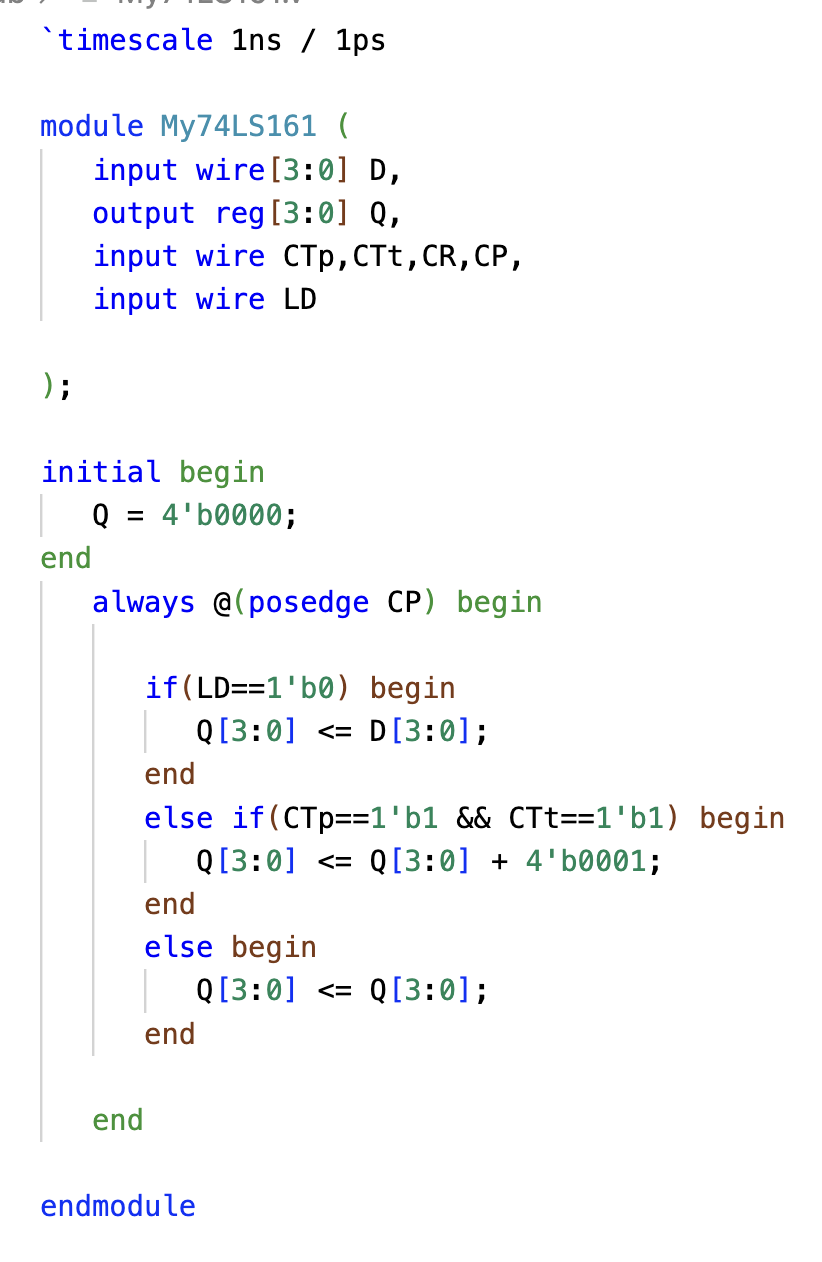
\includegraphics[width=0.5\textwidth]{1.png}
    \caption{\label{Lab12}74LS161}
    \end{figure}


\subsection*{任务2:利用74LS161完成时钟设计}

利用上面完成的74LS161模块进行数字时钟的设计,时钟可以对时、分、秒
的三个信息以BCD码的形式来显示,并且对设计的数字时钟进行验证.

利用verilog完成的数字时钟如下:
\begin{figure}[H]
    \centering
    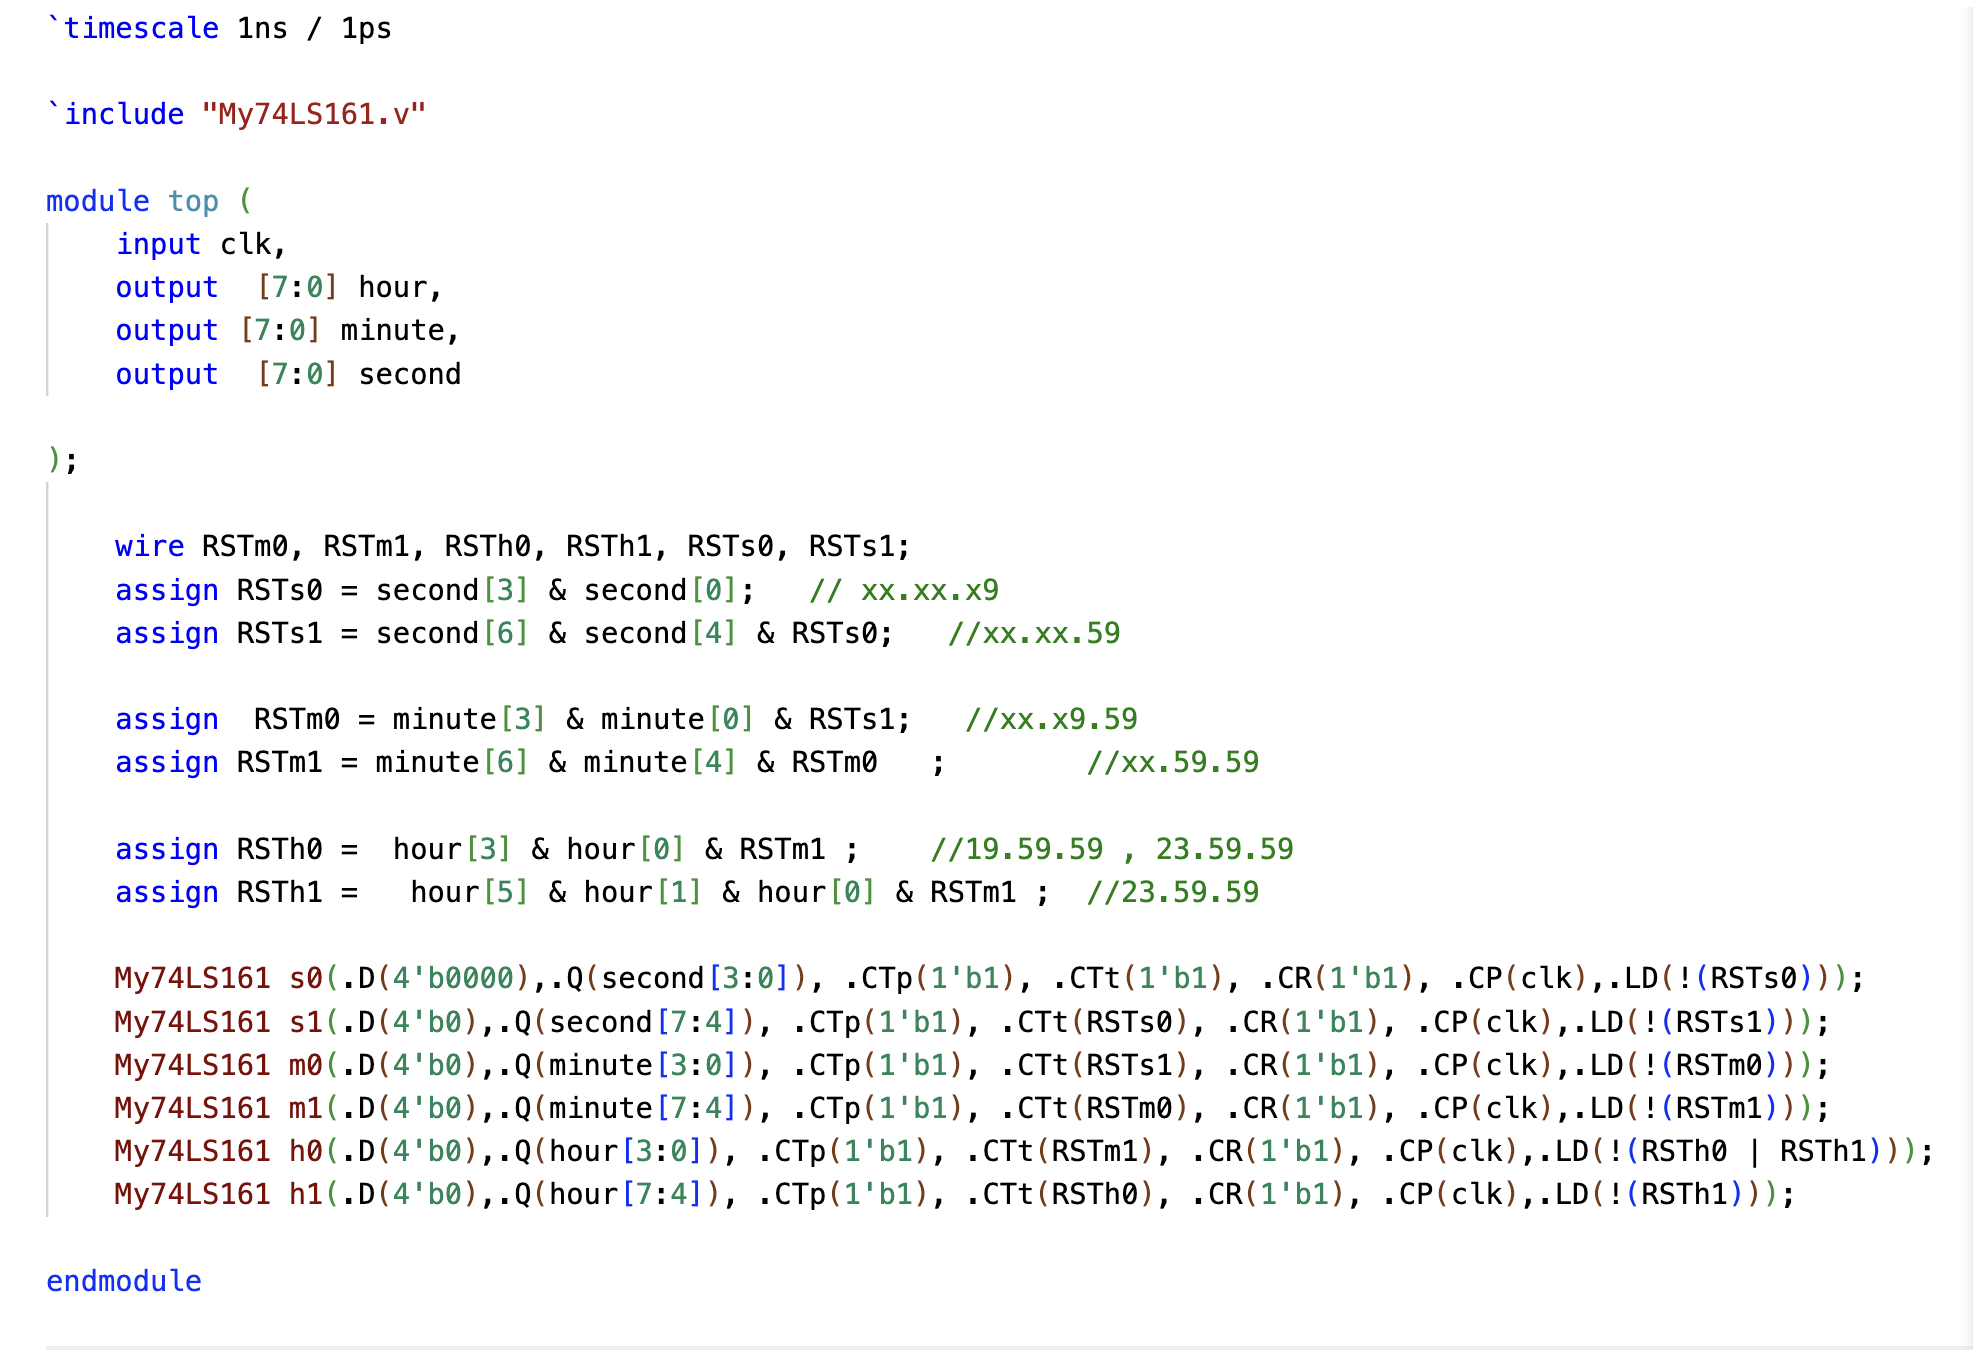
\includegraphics[width=1\textwidth]{2.png}
    \caption{\label{Lab12}数字时钟设计}
    \end{figure}

通过testbench对实验的测试结果进行分析,让数字时钟在clk信号的驱动下进行时间的显示.
testbench的代码如下:
\begin{figure}[H]
\centering
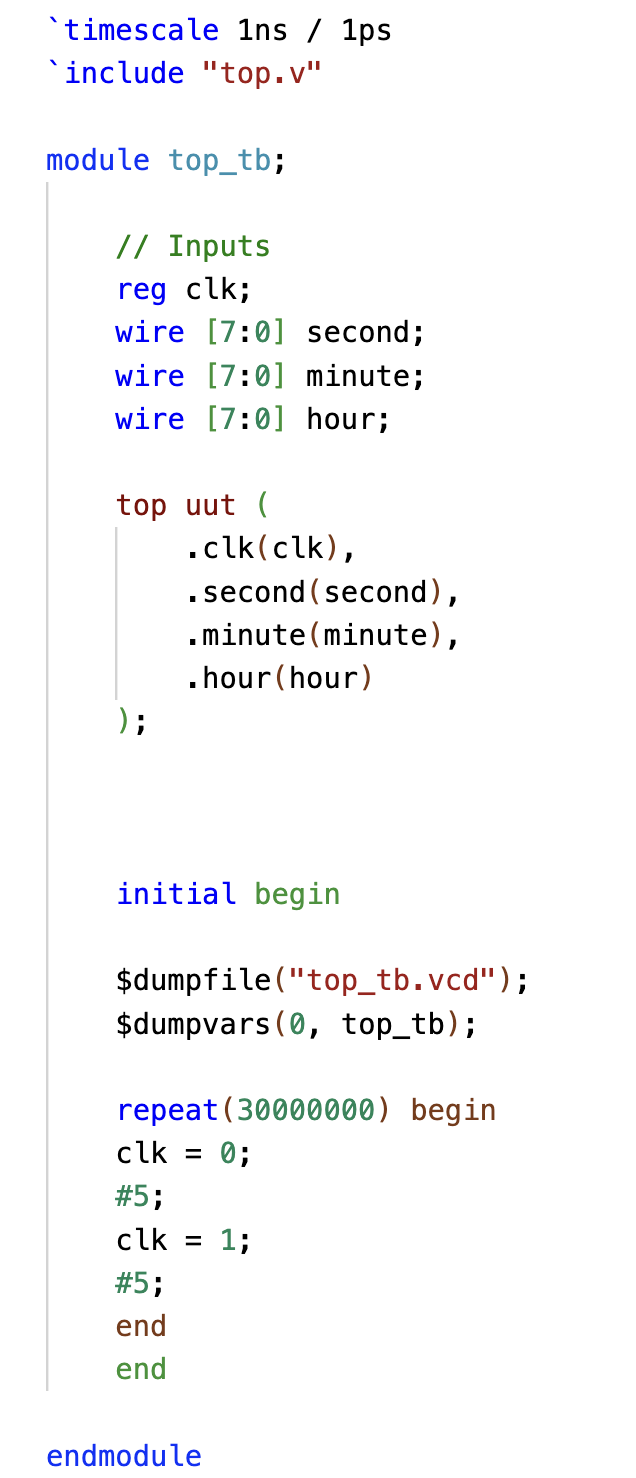
\includegraphics[width=0.4\textwidth]{3.png}
\caption{\label{Lab12}测试代码}
\end{figure}





\section*{二、实验结果与分析}

通过testbench波形图的分析对数字时钟进行测试.

\begin{figure}[H]
    \centering
    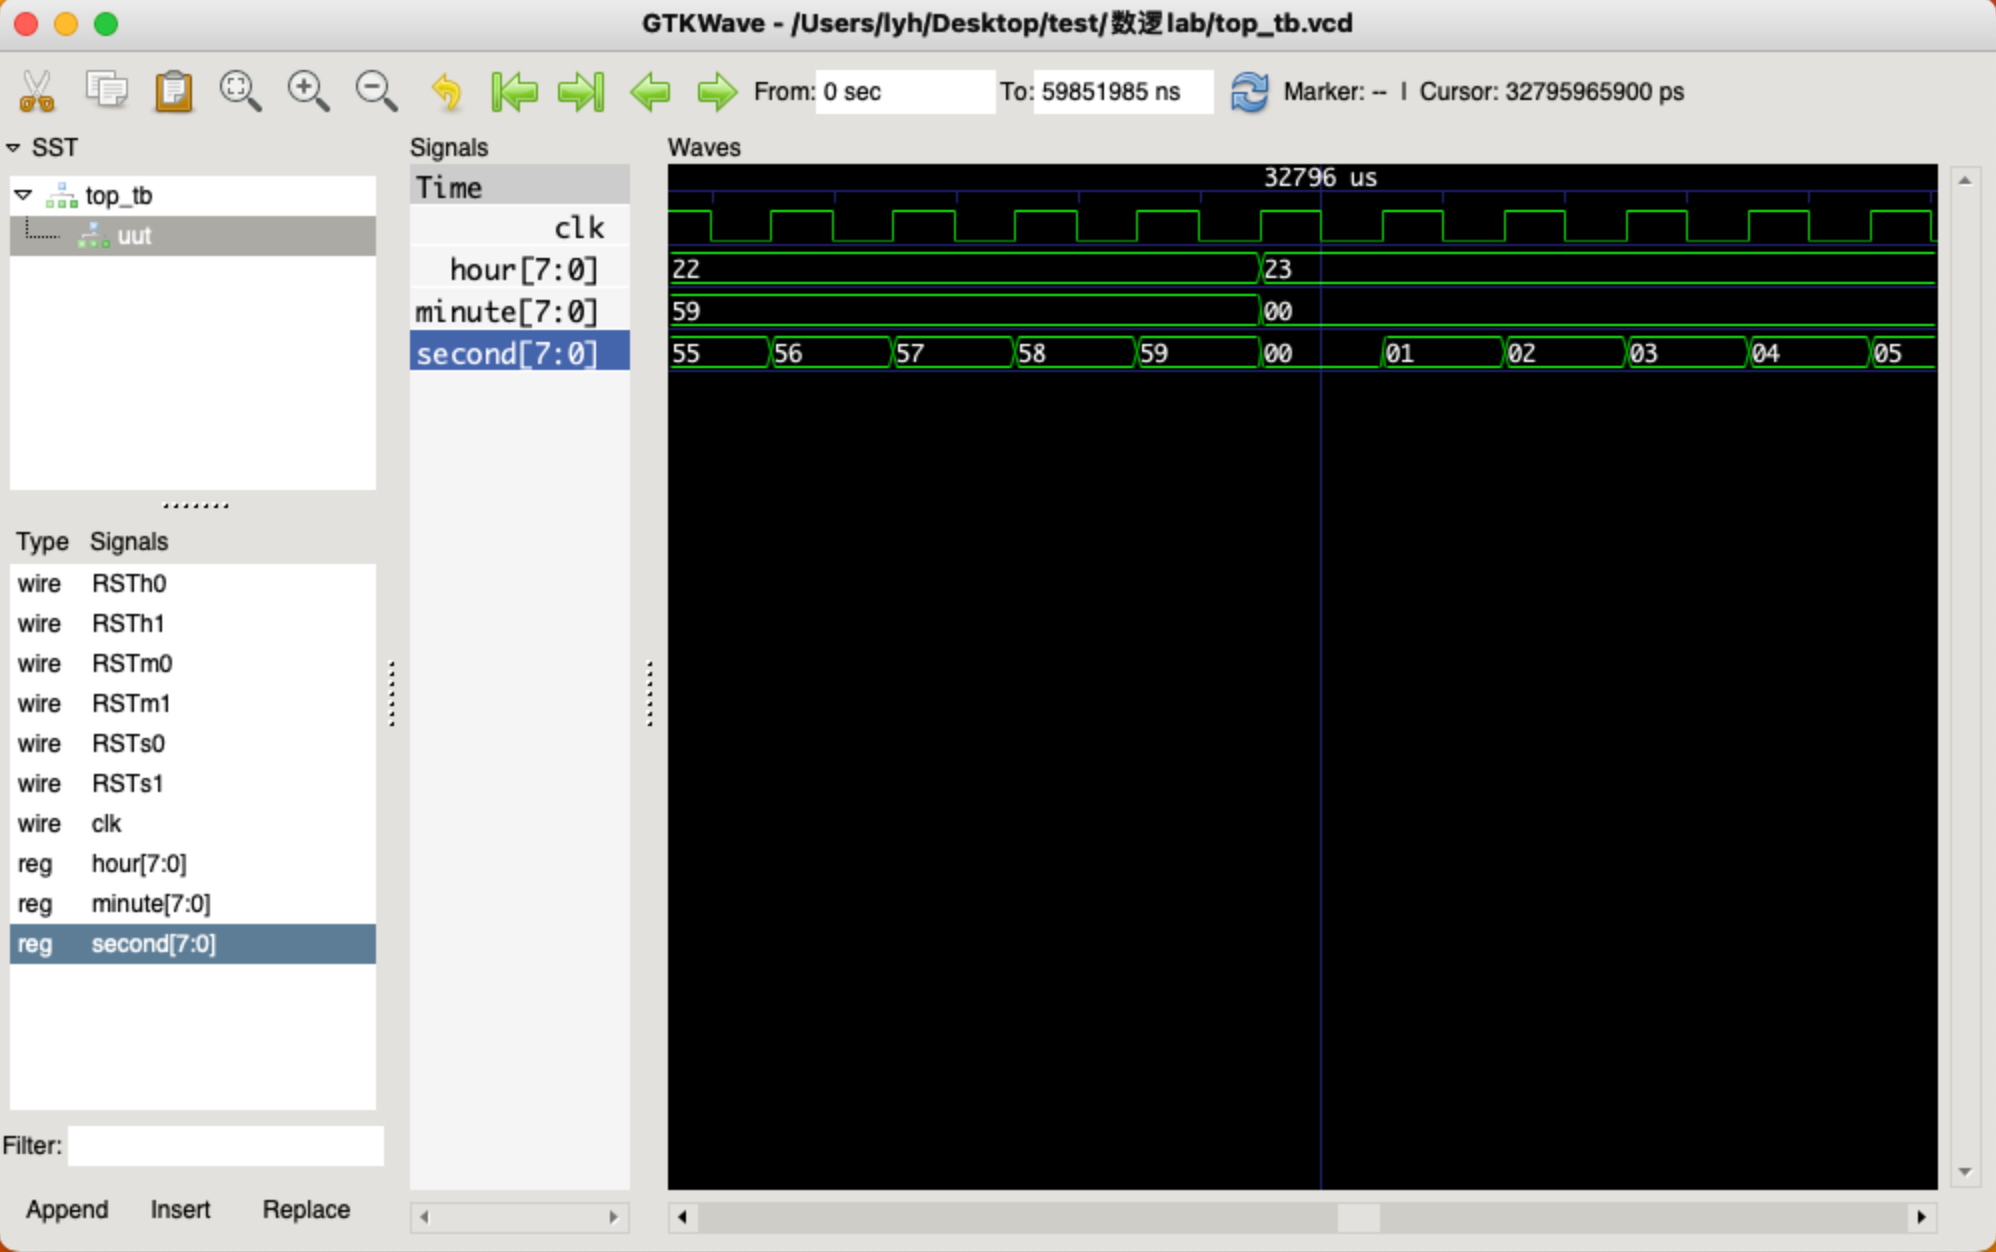
\includegraphics[width=1\textwidth]{4.png}
    \caption{\label{Lab12}波形分析}
    \end{figure}

    
    \begin{figure}[H]
        \centering
        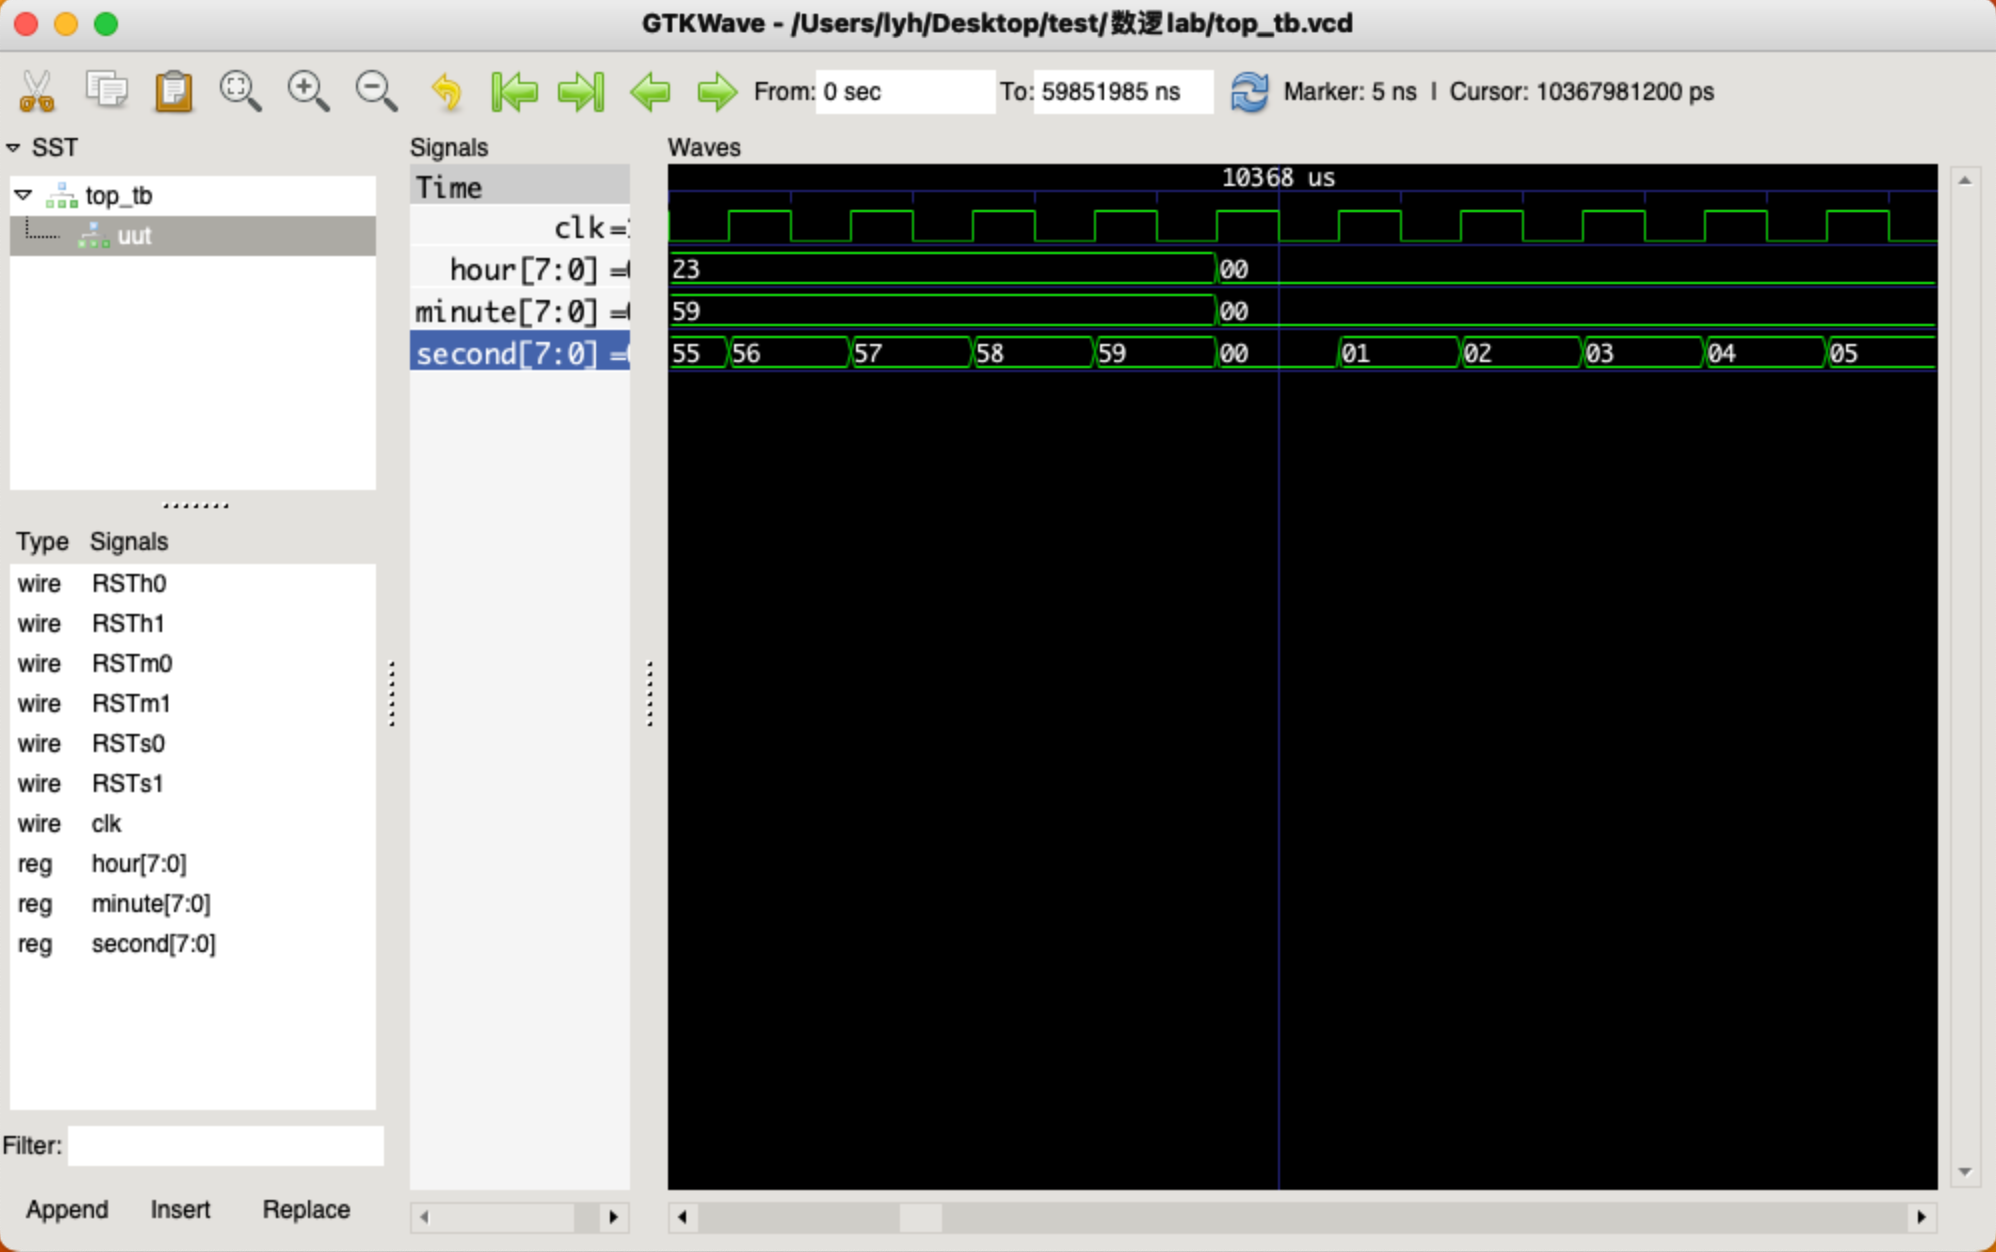
\includegraphics[width=1\textwidth]{5.png}
        \caption{\label{Lab12}波形分析}
        \end{figure}

        \begin{figure}[H]
            \centering
            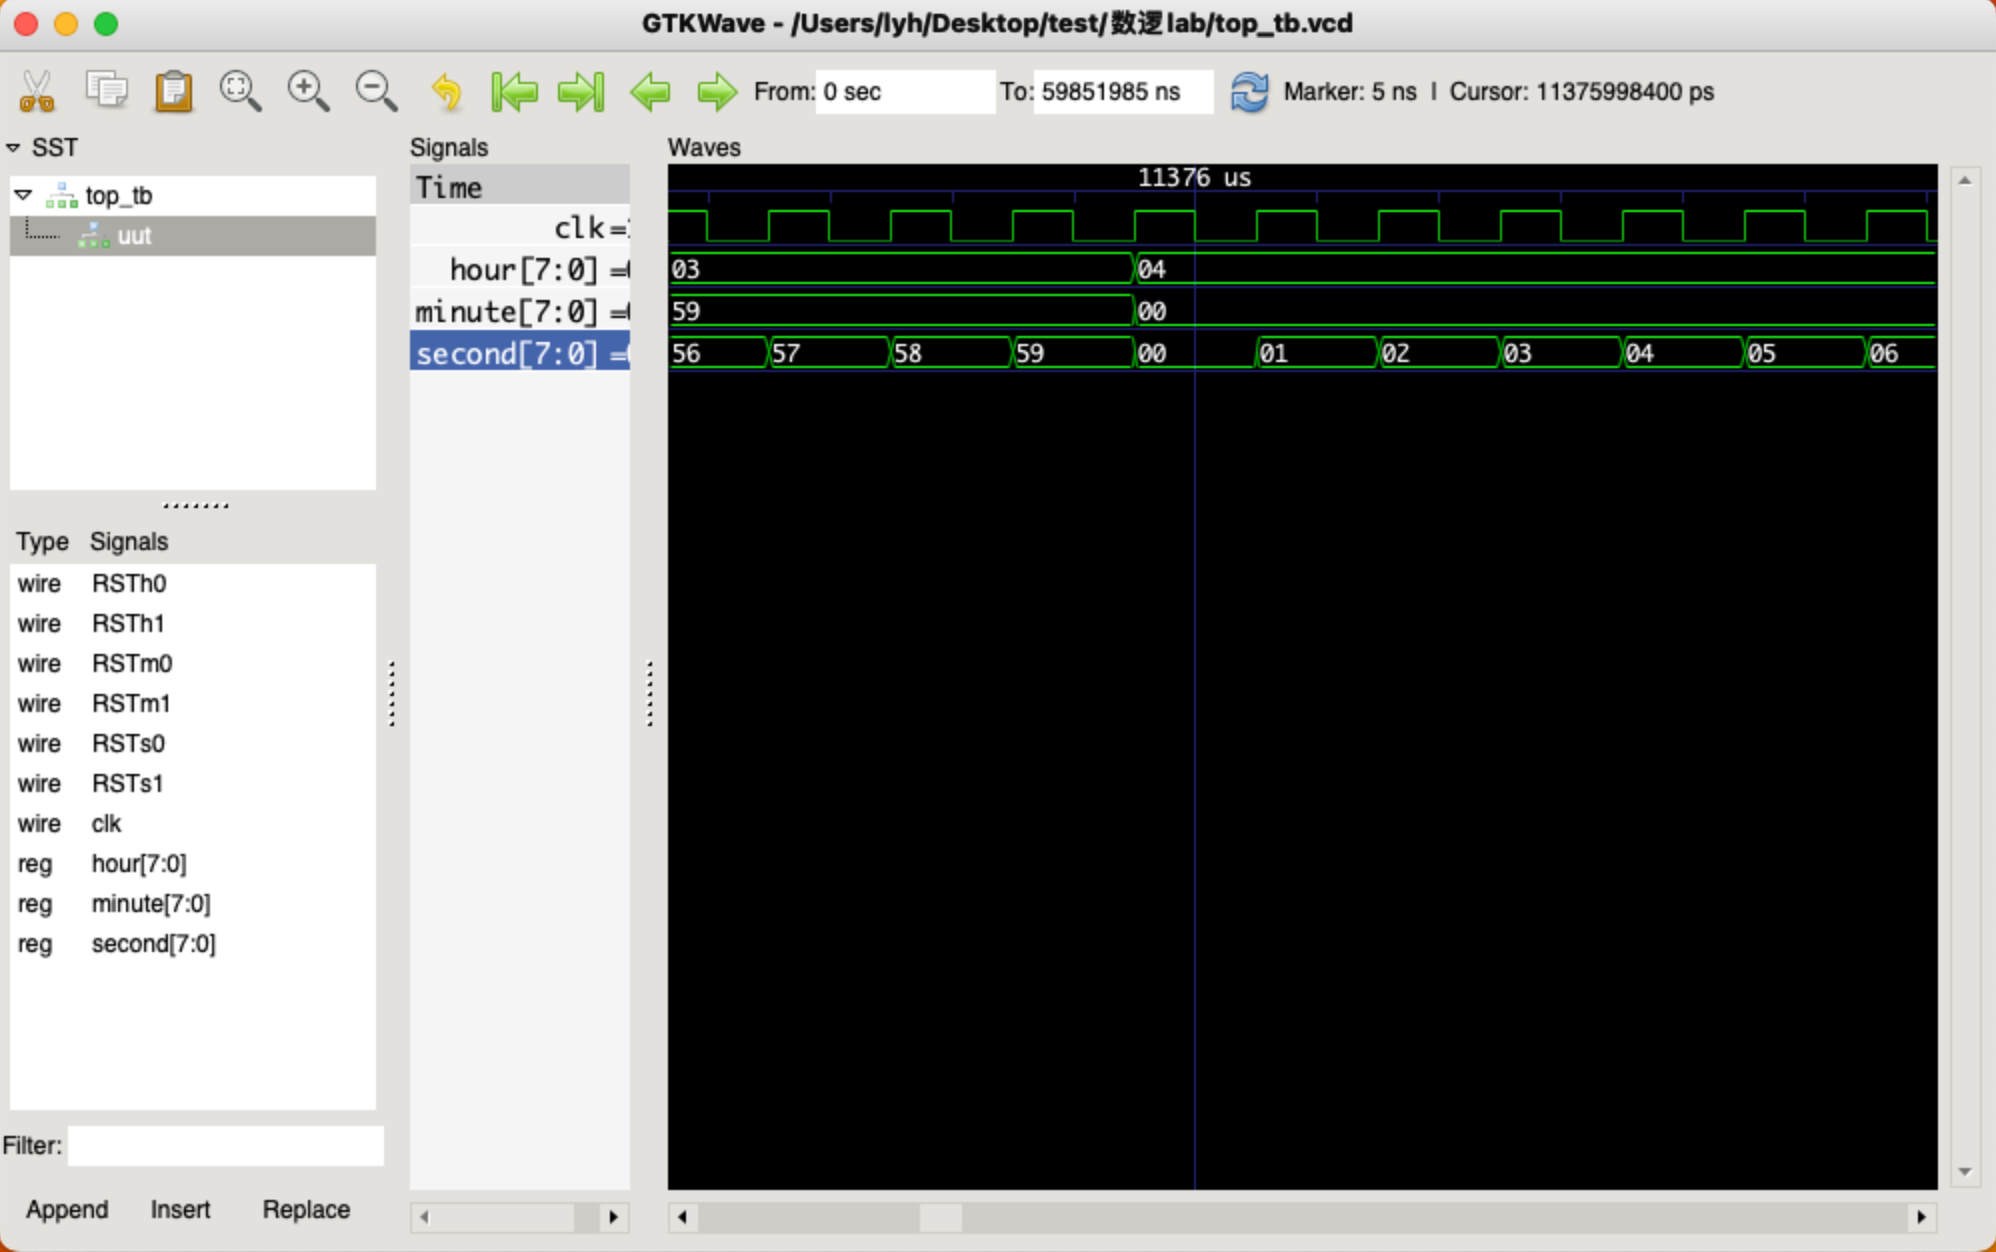
\includegraphics[width=1\textwidth]{6.png}
            \caption{\label{Lab12}波形分析}
            \end{figure}

所展示的波形图主要体现了对时钟进位时的正确性.

在第一张波形图中,有时间从22.59.59 -> 23.00.00 的过程,在top.v的代码中正确分析了
每一位的进位情况,可以显示出正确的时间.

第二张波形图中,可以看到时间从23.59.59 -> 24.00.00 的过程,正确完成了对hour最高位的进位判断.

第三张波形图,时间 03.59.59 -> 04.00.00, 是一个简单的信号进位的过程.

在全部的波形图中,这个数字时钟可以对时间进行正确的显示,可以看出代码完成的正确性.
            




\section*{三、讨论与心得}
由于疫情原因本次实验的内容全部是通过本地测试的方式来完成的,省去了下版验证的过程,因此一些
内容完成起来简单了很多.在这次实验中遇到的主要问题是不太清楚在什么位置对时钟的三个数字进行初始化,
因此进行了很多的尝试,最后才找到了正确的信号赋初始值的方法,成功完成了实验内容.


\end{document}